\documentclass{article}
\usepackage[utf8]{inputenc}

% MNRAS is set in Times font. If you don't have this installed (most LaTeX
% installations will be fine) or prefer the old Computer Modern fonts, comment
% out the following line
%\usepackage{newtxtext,newtxmath}
% Depending on your LaTeX fonts installation, you might get better results with one of these:
%\usepackage{mathptmx}
%\usepackage{txfonts}

% Use vector fonts, so it zooms properly in on-screen viewing software
% Don't change these lin es unless you know what you are doing
\usepackage[T1]{fontenc}
\usepackage{ae,aecompl}


%%%%%%%%%%%%%%% ADDITIONAL PACKAGES %%%%%%%%%%%%%%

% Only include extra packages if you really need them. Common packages are:
\usepackage{graphicx}	% Including figure files
\graphicspath{{Figures/}} % Set the path to the figures
\usepackage{amsmath}	% Advanced maths commands
\usepackage{amssymb}	% Extra maths symbols
\usepackage{breqn}
\usepackage{graphicx}
\usepackage{caption}
\usepackage{subcaption}
\usepackage{amsfonts, amsmath, amsthm, amssymb}
\usepackage{siunitx}
%%%%%%%%%%%%%%% ADDITIONAL COMMANDS %%%%%%%%%%%%%%

% Please keep new commands to a minimum, and use \newcommand not \def to avoid
% overwriting existing commands. Example:
%\newcommand{\pcm}{\,cm$^{-2}$}	% per cm-squared
\newcommand{\sz}{Sunyaev--Zel'dovich }

%%%%%%%%%%%%%%%%%%%%%%%%%%%%%%%%%%%%%%%%%%%%%%%%%%
%%%%%%%%%%%%%%%%%%%%%%%%%%%%%%%%%%%%%%%%%%%%%%%%%%




\title{A standardised environments for hippocampus and entorhinal cortex models}
\author{Clementine Domine and Rodrigo Carrasco}
\date{December 2021}

\begin{document}

\maketitle
\tableofcontents
\section{Introduction}
\subsection{Observation:}

After an in depth review of the literature of the hippocampus and entorhinal cortex models (See Excel table) , we made a number of observations.
The hippocampus is a complex organ that is given a great number of role. On one hand,t he hippocampus is known to be involved in the  consolidation of episodic memory to semantic memory from the hippocampus to the neocortex notably through the mechanism of replay.
On an other hand, it is famously known for its function in navigation through it ability to encode spatial information through a cognitive map of the environment.
Therefore we observe two main types of models and evidence. 
Models who are interested in the replay consolidation mechanism  during navigational task and models that replicated neural pattern and behaviour observed during Navigation task.It seems difficult to reconcile these two function of the hippocampus.However, we believe that creating an environment that allow to compare both types of models will guide us one the right track. \\



We pay a particular attention to the comparison that model make with experimental results. We first notice that the models results do not necessarly arise from the replication of the experimental behavioural data. We also note that models  results are compared to hand selected experimental evidence.
Indeed, there does not seems to be a consensus on the choice of experimental evidences. Moreover, there is a clear lack of counter evidence for each model. Considering the difficulty to access the validity of experimental neuroscience evidence from the multitude of experimental setting and setting, this seems natural.However, we believe that a single environment that allows the comparison to multiple set of evidences will solve these difficulty and push for a standardisation of the process. \\ 

Finally, we came a cross multiple coding style and methods for the models, which render difficult their understanding and comparison. \\

The above observation lead us to build this project.


\subsection{Inspiration:}

BenchMarks in the field of Machine learning are very common to assess the performance of models. It is certainly difficult to construct a measure as precise for neuroscience evidence. However, one can imagine an environment that allows the checking of the model to a great number of experimental evidences which will effectively acts a benchmark.This was attempted in the paper 'CCNLab: A Benchmarking Framework for Computational Cognitive Neuroscience'. We aim at creating a similar environment for hippocampus and entorhinal cortex models.

\subsection{Our Solution:}

We, therefore propose a standardised environments for hippocampus and entorhinal cortex models to answer all of the above limitations.
This model will allow the theoretical neuroscience to easily and consistently compare their model against the same set of experimental result This project was build to be collaborative and lasting. We hope that the framework will be simple enough to be adopted by a great number of neuroscientist. . We think that this framework will guide the path to the computational understanding of the hippocampal mechanism.

 This project will indirectly  push for a Standardisation of the field of neuroscience. Every hippocampal model integrated to this framework will have the same core structure.
In the same line, the methods and details of the experiment will be reported in a standardised manner. 

Finally, we think that this frame work will guide the theorist in building there model by clearly laying out the evidences they need to replicate. 




\section{Outline of the model}

The Code is constructed of two main piece,an Agent and an Environment. The agent can be thought of the animal performing the experiment and the Environment the experimental setting that the animal navigates These two class are allowed to interact with each other to reproduce the full experimental setting.

\subsection{The Agent}

The Agent is the first part of the model. The agent can be thought as the animal performing the task in the experiment. All agent types will be given a set of abilities that are summarised the core structure. The different model developed can be easily integrated to the core to finalise the agent type. that will guide the animal.
Multiple variable can be computed for the agents with respect to the needs of the model. Some examples are given bellow.

\begin{itemize}


\item Position
\item Velocity
\item Reward position
\item Visual cues
\item Head direction
\item Whiskers
\item Smell
\item Others…
\end{itemize}
Need to define an agent structure to interact with these environments.


\subsubsection{The models}

\begin{itemize}
 
    \item The Tolman-Eichenbaum machine: Unifying space and relational memory through generalization in the hippocampal formation \cite{whittington2020tolman}
    \item An oscillatory interference model of grid cell firing \cite{burgess2007oscillatory}
    \item A general model of hippocampal and dorsal striatal learning and decision making \cite{geerts2020general}
    \item Learning place cells, grid cells and invariances with excitatory and inhibitory plasticity \cite{weber2018learning}
    \item Flexible modulation of sequence generation in the entorhinal--hippocampal system \cite{mcnamee2021flexible}
    \item Prioritized memory access explains planning and hippocampal replay \cite{mattar2018prioritized}
    \item Coordinated hippocampal-entorhinal replay as structural inference \cite{evans2019coordinated}
    \item Modeling place cells and grid cells in multi-compartment environments: Entorhinal--hippocampal loop as a multisensory integration circuit\cite{li2020modeling}
\end{itemize}

\subsection{The Environment}

The Environment is the second main piece of the model. It aims at replicating the experimental environment. 
All of the environments are created based on the structure of core class. We begin with creating a simple 2 dimensional arena. We plan to implements more complex architectures such as a 3D environment,T-maze or a cylcle as shown in figure \ref{Env}. We will work toward improving the environment through out the project.
\begin{figure}
\centering
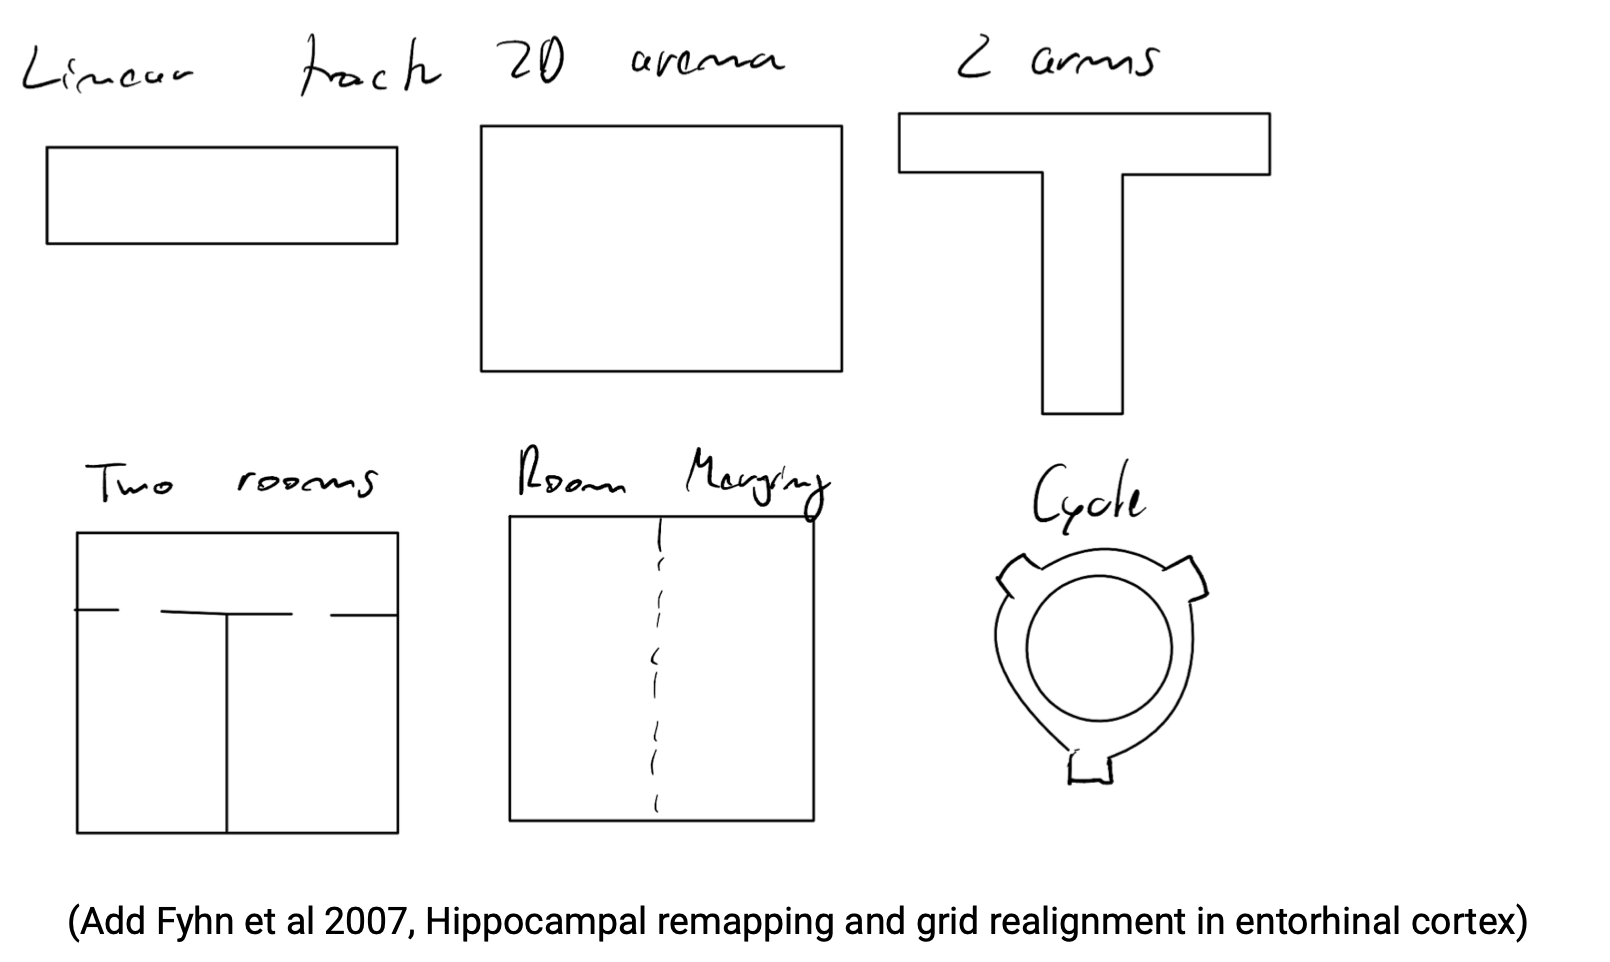
\includegraphics[scale=0.5]{Env.png}
\caption{ Sketch of the arenas.}
\label{Env}
\end{figure}


\subsubsection{The Experiment}

We use open source data of the experiment to replicate the experimental condition.
We use the following data sets:
\begin{itemize}
    \item  “Conjunctive Representation of Position, Direction, and Velocity in Entorhinal Cortex” Sargolini et al. 2006 Conjuctive cells \cite{sargolini2006conjunctive}

    \item “Hippocampus-independent phase precession in entorhinal grid cells”, Hafting et al 2008.
    \cite{hafting2008hippocampus}
    
\end{itemize}

\subsection{The Evidences}

We hope to assess the performance of the models against a set of selected evidences.

\textbf{Qualitative evidence}
\begin{itemize}
    \item Types of cells: Grid, place, band, etc
\item Presence of replay
\item Phase precession
\item Is the model biologically connected?
\item Is the model biologically plausible?
\end{itemize}

\textbf{Quantitative evidence}
\begin{itemize}
\item Learning time scales
\item Replay directions under different conditions
\item Animal trajectories
\end{itemize}

Users might use only some of the available experiments and comparison depending on the capabilities of the models
We want to reinstate that this wont constitute an objective judgement of the quality of a model to replicate the brain mechanism. This only allows an objective and complete comparison to the current evidences in the field.

\section{Masters Project Idea}

We are offering a Master student interested in working in the field of computational neuroscience to join us on this project. The main duties would involve
\begin{itemize}
\item Implement an hippocampal and entorhinal cortex models of your choice.

\item Compare its results to real experimental data.

\item Work on improving the environment 
(3D, Simulus, T-maze, separate rooms)


\end{itemize}
This project will developped the student neurosceince knowldge and coding skills.Any significant contribution will be considered during the publication process. We hope you will want to join us !

\bibliographystyle{hieeetr} %hieeetr allows eprint field

%{\small
\bibliography{references}

\end{document}
